\documentclass[12pt,a4paper]{article}

\usepackage[utf8]{inputenc}
\usepackage[T1]{fontenc}
\usepackage{lmodern}
\usepackage[margin=1in]{geometry}
\usepackage{setspace}
\onehalfspacing
\usepackage[round]{natbib}
\usepackage{amsmath}
\usepackage{amsthm}
\usepackage{graphicx}
\usepackage{booktabs}
\usepackage{adjustbox}
\usepackage{caption}
\usepackage{tikz}
\usetikzlibrary{positioning,arrows.meta,calc,fit}
\usepackage{microtype}
\usepackage[hidelinks]{hyperref}

\theoremstyle{definition}
\newtheorem{proposition}{Proposition}

\title{Promises Made in Public: Venue Congruence and Generation Z's Ethical Voice After Ideological Contract Breach}
\author{[AUTHORS TBD]$^{1*}$ \\ $^{1}$ [Affiliation TBD] \\ \texttt{[CORRESPONDING EMAIL TBD]}}
\date{}

\begin{document}
\maketitle

\begin{abstract}
\noindent Research on Generation Z and workplace ethics has mostly asked whether this cohort holds stronger ethical values than earlier ones, a premise that meta-analytic and critical reviews of generational research do little to support. This conceptual paper asks a different question: when employees conclude that their employer has broken an ethical commitment, where do they take the complaint? Grounded in psychological contract theory, in particular its account of ideological currency, and in the exit-voice-loyalty framework, the paper develops a venue congruence model. It introduces promise publicity, the extent to which an employee's understanding of the employer's ethical obligations was formed through communication addressed to the public, and proposes that breaches of publicly made ethical promises are more likely to be felt as violations and more likely to be voiced publicly than internally. Perceived internal voice safety is proposed as the boundary condition that determines whether felt violation is expressed inside the organization, taken public, or turned into exit or silence. Two rival propositions separate a cohort explanation of the pattern often attributed to Generation Z from a career-stage explanation based on newcomer status. The paper reports no data; all five propositions are offered for empirical testing, and the discussion outlines designs and measures for doing so.

\medskip
\noindent\textit{Keywords:} Generation Z, workplace ethics, ideological psychological contract, employee voice, whistleblowing, generational cohort
\end{abstract}

\section{Introduction}
When an employee concludes that the organization has broken an ethical commitment, the concern can travel in several directions. It can go to a supervisor or an ethics office, where it may be fixed quietly. It can go to the public, through social media or the press, where it may damage the organization's reputation but also force change. It can leave with the employee, or it can stay unspoken. Which of these happens matters to the organization, which learns about problems only through the first route, and to the employee, who faces different risks on each. Hirschman's classic analysis made a related point about organizations in decline: members who speak tell the organization what has gone wrong, while members who leave signal only that something has \citep{hirschman1970exit}. Research on voice and silence has shown that employees often keep concerns to themselves because speaking up feels risky or pointless \citep{morrison2000organizational,milliken2003exploratory}, and research on whistleblowing has shown that people who disclose outside the organization differ from those who report inside it in their circumstances and in the retaliation they suffer \citep{dworkin1998internal}. The direction an ethical complaint takes is a workplace ethics question in its own right.

Discussions of Generation Z at work often start from a different question: whether this cohort cares more about ethics than earlier ones. The evidence gives that premise little support. A large time-lag study did not find that a recent cohort placed more weight on altruistic work values than its predecessors \citep{twenge2010generational}, meta-analytic work has found generational differences in work attitudes to be small \citep{costanza2012generational}, and critical reviews argue that differences attributed to generations are hard to separate from age, period, and career stage and are often better explained by those factors \citep{lyons2014generational,rudolph2021generations}. Building a model of Generation Z's workplace ethics on an assumed difference in values would rest on weak ground.

Two terms need to be pinned down before going further. By workplace ethics we mean the standards of right conduct that govern how an organization and its members treat employees, customers, and others affected by their work, together with the commitments an organization makes about honoring those standards. Research on behavioral ethics has studied how individual, group, and organizational factors shape conduct against such standards \citep{trevino2006behavioral}; our focus is narrower, on what employees do when they believe the organization itself has fallen short of a commitment it made. By Generation Z we mean the cohort that followed the Millennials into the labor market. The birth years used to mark its boundaries differ from source to source, and critics note that such boundaries are set by convention rather than derived from theory \citep{rudolph2021generations}. We therefore use the label descriptively and make no assumption that it marks a group with shared psychological traits. Whether it marks anything that matters for ethical voice is one of the questions the model is built to test.

A more tractable question concerns venue rather than values. A UK practitioner survey reported that its youngest respondents were less likely than older ones to say they would raise concerns with their employer, yet more likely to say they would post about workplace problems on social media or contact journalists \citep{protect2025talkin}. The survey was not peer reviewed and measured intentions at one point in time, so it cannot tell us whether the pattern reflects cohort, age, or the simple fact that young workers tend to be newcomers in junior roles. It does describe a tension worth explaining: reluctance to speak inside combined with readiness to speak outside. Existing theory offers pieces of an explanation. Psychological contract research explains how broken ethical commitments are experienced \citep{thompson2003violations}, and the exit-voice-loyalty tradition explains how people choose among responses to organizational decline \citep{hirschman1970exit,turnley1999impact}. Neither addresses why an employee would choose a public venue over an internal one.

This paper develops a model to address that question. Our central argument is that the venue in which an ethical promise was made shapes the venue in which its breach is contested. Organizations promote what they stand for as employers to outside audiences through employer branding \citep{backhaus2004conceptualizing}, and job seekers respond to signals about corporate social performance \citep{jones2014why}. We assume, without claiming it has been shown, that for many recruits an employer's ethical commitments are therefore first met in public form. We introduce promise publicity to capture this and propose that breaches of publicly made ethical promises are more likely to be felt as violations and more likely to be voiced publicly, a relationship we call venue congruence. Internal voice safety sets the boundary on this effect. Where neither venue seems viable, we expect exit or silence. Finally, rather than assuming that Generation Z behaves differently, we state two rival propositions, one attributing the pattern to cohort and one to career stage, and outline how research could decide between them.

The paper makes three contributions, each of which remains to be tested.

\begin{itemize}
\item It adds promise publicity to psychological contract theory as a feature of how ideological contracts are formed. Prior work has established that contracts form partly from pre-entry schemas and recruitment messages \citep{rousseau2001schema} and that ideological breach triggers compensatory or corrective responses \citep{yang2022going,deng2023serving}; we propose that the public or private origin of the ethical promise affects both the intensity of violation and the venue of the response.
\item It extends exit-voice-loyalty reasoning, which organizational research has applied mainly to internal voice \citep{morrison2014employee}, by treating the choice between internal and public ethical voice as the outcome to be explained, with internal voice safety as its boundary and exit and silence as the alternatives when neither venue appears viable. Studies of ethical culture have shown that culture relates to internal versus external responses \citep{kaptein2011inaction}; our model adds the promise's origin as a second influence on that choice.
\item It recasts the Generation Z question as a contest between rival propositions, following critics who argue that generational labels are often confounded with age and career stage \citep{rudolph2017considering,parry2011generational}, and it differs from the closest existing study of online whistleblowing and ideological contracts \citep{yang2026managing} by modeling the internal alternative, the exit and silence outlets, and the cohort question.
\end{itemize}

\section{Literature Review}
The model draws on three literatures that have developed largely apart. We review each for what it establishes and what it leaves open, and we close by identifying the connection none of them makes.

\subsection{Generations at Work: What the Evidence Supports}

The sociological idea of a generation comes from \citet{mannheim1952problem}, who argued that people born in the same period share a location in historical time and may, if they are exposed to the same formative events, develop a shared outlook. Mannheim did not claim that birth cohorts automatically become generations in this richer sense; shared location was a precondition, not a guarantee. Management research has often skipped that qualification and treated cohort labels as if they carried stable traits.

The empirical record on generational differences at work is modest. A large time-lag study of American high school seniors found that the value placed on leisure rose across cohorts and work centrality fell, but it did not find that the most recent cohort it studied placed more weight on altruistic work values such as helping others or contributing to society \citep{twenge2010generational}. That finding is worth keeping in mind, because popular accounts of younger workers often assume the opposite. A meta-analysis of generational differences in job satisfaction, organizational commitment, and turnover intentions concluded that the differences were small or close to zero in most comparisons \citep{costanza2012generational}. Reviews of work values and of the wider workplace literature describe the evidence as mixed and largely descriptive, and both point to a recurring difficulty in separating the effect of cohort from the effects of age and period \citep{parry2011generational,lyons2014generational}.

A more critical line of work questions whether generations are a useful explanatory category for individual behavior at all. \citet{rudolph2017considering} proposed a lifespan developmental perspective as an alternative, arguing that the processes usually attributed to generation are better understood as developmental and contextual. \citet{rudolph2018leadership} reached a similar conclusion for leadership research, and \citet{rudolph2021generations} set out a series of common claims about generations that they argued are not supported by evidence. A different response to the same problem is to treat generation as an identity that becomes relevant in some organizational situations and not others \citep{joshi2010unpacking}, which shifts attention from what a cohort is like to when cohort membership matters. In our reading, research that links Generation Z specifically to workplace ethics is thinner still, and much of what circulates comes from practitioner surveys rather than peer-reviewed studies.

For our purposes, this literature establishes a caution rather than a finding. It gives little support for building a model on the premise that Generation Z holds stronger ethical values than earlier cohorts. It leaves open a narrower question that it has rarely asked: whether cohorts differ in the channels through which they act on ethical concerns, and whether any such difference survives once age and career stage are taken into account.

\subsection{Ideological Psychological Contracts and Responses to Breach}

Psychological contract research began with the insight that employees hold beliefs about mutual obligations that go beyond any formal agreement \citep{rousseau1989psychological}. Later work traced how these beliefs form, locating their origins partly in pre-entry schemas and in promises communicated through the recruitment and socialization process \citep{rousseau2001schema}. A central distinction separates breach, the perception that an obligation has not been met, from violation, the emotional response of anger and betrayal \citep{morrison1997employees}. Longitudinal evidence showed that breach was more likely when newcomers had little interaction with organizational agents before being hired, and that breach turned into more intense violation when it was attributed to deliberate reneging and handled unfairly \citep{robinson2000development}. A meta-analysis confirmed that breach is associated with a wide range of attitudes and behaviors and identified violation and mistrust as affective links in that chain \citep{zhao2007impact}.

\citet{thompson2003violations} widened the theory by proposing ideological currency: commitments by the organization to a cause or principle that the employee values and that benefits parties beyond the employee. This extension brought ethical commitments inside the psychological contract. A recent review lists ideological currency among the directions in which the field needs further research \citep{coyleshapiro2019psychological}. Empirical work on how employees respond to ideological breach has begun to accumulate. One study found that breach prompted pro-social rule breaking, which the authors interpret as corrective behavior on behalf of the ideology \citep{yang2022going}. Another, in a hospital setting, found that ideological breach led employees to ruminate and then to reaffirm their own values through compensatory effort on behalf of the cause \citep{deng2023serving}.

These studies examine responses directed at the work itself or at the cause. Earlier research on non-ideological contracts looked at responses directed at the organization: managers who experienced violations reported more exit, voice, and neglect and less loyalty, and the availability of attractive job alternatives moderated the link to exit \citep{turnley1999impact}. What this literature does not examine is the channel through which an employee who wants to act on a broken ethical commitment chooses to do so, nor whether that choice depends on how the commitment was communicated in the first place. The formation research tells us that promises are conveyed through many channels, and the breach research tells us that how employees interpret a breach shapes the emotional response, yet the two have not been joined to ask whether the public or private origin of an ethical promise changes what employees do when it is broken.

\subsection{Ethical Voice, Silence, and the Choice of Channel}

Behavioral ethics research asks how people in organizations come to act rightly or wrongly \citep{trevino2006behavioral}. Two streams within and alongside it address what employees do when they see something wrong. The voice stream studies upward communication of concerns and suggestions and its opposite, silence \citep{morrison2014employee,morrison2023employee}. It has shown that silence can be widespread and collectively reinforced \citep{morrison2000organizational} and that the decision to speak rests on judgments about safety and efficacy. The whistleblowing stream studies disclosure of wrongdoing to parties who can act on it, and its standard definition includes disclosures both inside and outside the organization \citep{near1985organizational}. A book-length synthesis summarized decades of this research \citep{miceli2008whistleblowing}, and a review organized the field around who blows the whistle, about what, how, why, and to whom \citep{culiberg2017evolution}.

The question of channel appears most directly in the whistleblowing stream. A comparison of dismissed whistleblowers found that those who went outside the organization had shorter tenure and stronger evidence than those who reported internally, were more effective in changing practices, and suffered more extensive retaliation \citep{dworkin1998internal}. A study of intended responses to observed wrongdoing found that stronger ethical cultures were associated with less intended inaction and less intended external whistleblowing, and with more intended internal reporting \citep{kaptein2011inaction}. A meta-analysis found that personal, situational, and wrongdoing characteristics predicted whistleblowing intentions more strongly than actual whistleblowing \citep{mesmermagnus2005whistleblowing}, a reminder that stated intentions are a weak guide to behavior.

Voice research offers a further distinction that bears on ethical concerns. Voice can promote a new idea or it can object to something harmful that is already happening, and the second kind, prohibitive voice, carries more interpersonal risk because it implies criticism of current practice or of the people responsible for it. In a two-wave study, psychological safety was more strongly related to prohibitive than to promotive voice \citep{liang2012psychological}. Raising an ethical objection to an employer's conduct is a clear case of prohibitive voice. The same research tradition also shows that silence is not a single state: employees may withhold concerns because they have given up, because they fear the consequences, or because they wish to protect others \citep{vandyne2003conceptualizing}. These distinctions matter for the model because they imply that the internal channel is least attractive precisely for the kind of concern at issue here.

Social media have added a new external channel. Commentators have pointed out that employees can now reach large audiences with their views of the employer, for better or worse \citep{miles2014employee}, and a study in business ethics examined how an organization's social media strategy and policy affect employees' sensitivity to the risks of whistleblowing through social media \citep{xiao2022employee}. Communication research explains part of the channel's reach: social media make content visible to wide audiences and keep it available long after it is posted \citep{treem2013social}. This work treats the social media channel as a risk to be managed. It does not ask what makes the channel attractive to a given employee after a given breach.

\medskip

Across the three literatures, the missing link is the relationship between where an ethical promise is made and where its breach is contested. Generational research has focused on value levels and has not modeled channel choice. Ideological contract research has studied how employees feel and what they do for the cause after breach, but has not examined the venue of their response or the venue of the original promise. Voice and whistleblowing research has distinguished internal from external channels and has identified ethical culture and safety as influences on the choice, but has not asked whether the promise's origin matters. The nearest existing work combines ideological contract and signaling reasoning to study employees' online whistleblowing about their employers' public stances on social issues, with the practical aim of guiding internal communication about those stances \citep{yang2026managing}. It shares our interest in public promises and public responses. It does not model internal voice safety as a boundary, exit and silence as alternative outlets, or the rival cohort and career-stage explanations that the Generation Z question requires. Those are the elements our model adds.

\section{Theoretical Framework and Approach}
\subsection{Approach}

This is a conceptual article. It builds a model from existing theory and states its claims as propositions, which are statements about relationships among constructs that are meant to be tested rather than claims that have already been confirmed. Among the designs available for conceptual work, ours is closest to what \citet{jaakkola2020designing} calls a model paper, one that specifies constructs and the relationships among them. We follow the view of \citet{whetten1989constitutes} that a theoretical contribution must say which factors matter, how they are related, and why the proposed relationships should hold, and we adopt the propositional style that \citet{cornelissen2017developing} describes as suited to explaining variance in an outcome across conditions. Throughout, we separate three kinds of statement. The first reports what cited studies found. The second reports what cited theories argue. The third, flagged each time, is our own reasoning, which has not yet been tested.

\subsection{Psychological Contract Theory and Ideological Currency}

A psychological contract is an individual's belief about the reciprocal obligations between that individual and the employing organization \citep{rousseau1989psychological}. The belief need not match what the organization intended, and it need not be written down. What makes it a contract, in the psychological sense, is that the employee believes a promise was made and that something was given in return. \citet{rousseau2001schema} argued that these beliefs form partly before entry, from schemas the person already holds about employment and from promises communicated through words and actions during recruitment and early socialization. That point about formation matters for our model, because it treats where and how an obligation was communicated as part of the contract itself.

\citet{thompson2003violations} extended the theory by adding ideological currency to the transactional and relational currencies already recognized. An ideological contract involves the employee's belief that the organization has made a credible commitment to pursue a valued cause or principle, one that benefits parties beyond the employee. When such a commitment is broken, the employee has lost more than a personal benefit, because a principle the employee cared about has been abandoned. This is the closest established construct to what we mean by an employer's ethical commitments, and it is why we ground the model here rather than in a general account of fairness. Psychological contract theory also supplies the distinction between breach, the cognitive judgment that an obligation has gone unmet, and violation, the emotional experience of anger and betrayal that may or may not follow \citep{morrison1997employees}. That distinction lets us ask what turns a noticed breach into a felt violation.

\subsection{The Exit-Voice-Loyalty Framework and the Question of Venue}

Hirschman's framework concerns how members respond when an organization they belong to deteriorates. They can leave, which is exit, or they can try to change it from within, which is voice; loyalty holds exit back and gives voice time to work \citep{hirschman1970exit}. Organizational researchers later added neglect and arranged the responses along two dimensions, active versus passive and constructive versus destructive \citep{farrell1983exit}, and showed that satisfaction, investment, and the quality of alternatives shape which response people choose \citep{rusbult1988impact}. \citet{turnley1999impact} connected this tradition directly to psychological contracts, reporting that managers who experienced contract violations reported more exit, voice, and neglect and less loyalty.

The framework is a theory of response choice after something has gone wrong, which is exactly the problem we address. Its limitation for our purpose lies in how voice has been carried into organizational research. Hirschman's own notion of voice was broad: any attempt to change a state of affairs rather than escape it, whether by petitioning management, appealing to a higher authority, or protesting in ways meant to rally outside opinion. Organizational behavior research later narrowed the construct, typically defining voice as upward communication of concerns or suggestions to someone with authority inside the organization \citep{morrison2014employee}, while disclosures to outside parties were studied separately as external whistleblowing. The result is that neither literature asks what makes an employee choose one venue over the other after the same breach. A complaint raised with a supervisor and a complaint posted to a public audience differ in who hears them and in the risk they carry for the employee. We therefore keep the framework's core logic, in which the availability and expected effectiveness of voice govern whether people stay and speak or leave, and we treat venue as a choice within voice that needs its own explanation.

\subsection{Why These Two Theories}

Several alternatives were considered and set aside. Signaling theory has been used to explain why job seekers are drawn to socially responsible employers \citep{jones2014why}, and it has been combined with ideological contract reasoning to study online whistleblowing about corporate social advocacy \citep{yang2026managing}. It is well suited to explaining how public claims create expectations, but it says little about what employees do after those expectations are disappointed, which is our focal question. Social exchange reasoning in general underlies psychological contract theory, but on its own it is too broad to generate predictions about channel choice. Generational theory, traced to \citet{mannheim1952problem}, is not used here as a causal theory, for reasons developed in the literature review: its workplace applications have weak empirical support, and we prefer to treat the generational question as something to be tested against a competing explanation. Psychological contract theory tells us what an ethical promise is and why its breach can be felt as betrayal. The exit-voice-loyalty framework tells us how people choose among responses. The two fit together because the second begins where the first ends.

\subsection{Scope Conditions}

The model applies to employees of organizations that make ethical commitments that employees can perceive, whether through public statements, recruitment messages, or interpersonal assurances. It concerns breaches of those commitments as the employee perceives them; it does not assume that a breach occurred in any objective sense. It is not a model of whistleblowing on crime in general, where legal duties and protections change the calculus, although it overlaps with that literature. It also assumes that public channels are available to the employee at a cost that is not prohibitive; where public criticism of an employer carries severe legal or social penalties, we expect the model's predictions about public voice to weaken, a point we return to in the discussion.

\section{Conceptual Model and Propositions}
\subsection{Overview}

Figure~\ref{fig:model} summarizes the venue congruence model. Its starting point is an employee's perception that the employer has broken an ethical commitment, which we call ideological contract breach. The model proposes that such a breach is more likely to be felt as a violation when the commitment was learned through the employer's public communication, and that the same feature of the promise, its publicity, pushes the employee's response toward public rather than internal venues. Internal voice safety sets the boundary: where raising concerns inside feels safe and worthwhile, the internal channel is expected to absorb much of the response; where it does not, the response is expected to go public or, when the promise was private, to turn into exit or silence. The final proposition concerns Generation Z and is stated as two rival accounts. Every arrow in the figure is a proposition, and none has been tested.

\begin{figure}[htb]\centering
%% FIGURE-SPEC type=framework
%% DESC: drawn directly in TikZ (no image model): breach -> felt violation -> venue group (internal, public voice) and withdrawal group (exit, silence); promise publicity dashed to P1 and P2; internal voice safety between the two response paths, dashed to P3 and P4; dotted rival-accounts box (P5a/P5b) to promise publicity and internal voice safety
\resizebox{\linewidth}{!}{%
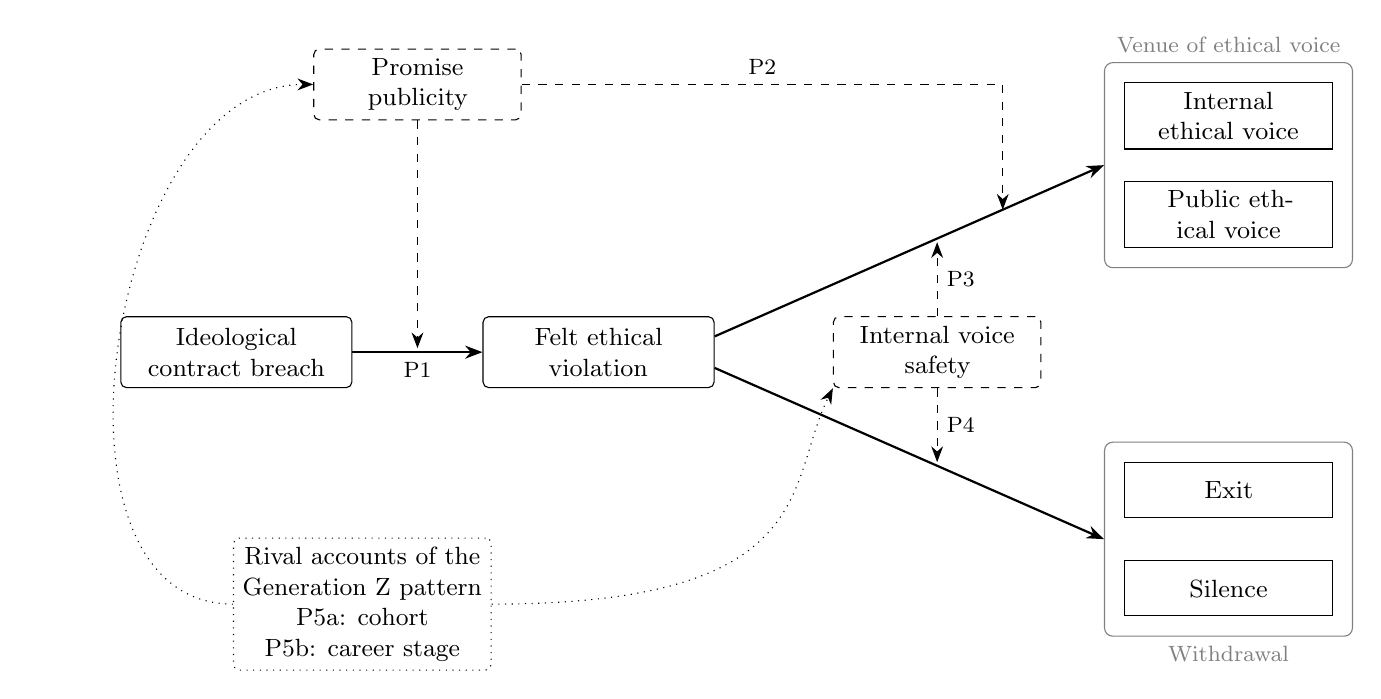
\begin{tikzpicture}[font=\small, box/.style={draw, rounded corners=2pt, align=center, minimum height=9mm, text width=27mm, fill=white}, mod/.style={draw, dashed, rounded corners=2pt, align=center, minimum height=8mm, text width=24mm, fill=white}, resp/.style={draw, align=center, minimum height=7mm, text width=24mm, fill=white}, grp/.style={draw, gray, rounded corners=3pt, inner sep=2.5mm}, arr/.style={-{Stealth[length=2.2mm]}, thick}, marr/.style={-{Stealth[length=2mm]}, dashed}, rarr/.style={-{Stealth[length=2mm]}, dotted}]
\node[box] (icb) at (0,0) {Ideological\\contract breach};
\node[box] (fev) at (4.6,0) {Felt ethical\\violation};
\node[resp] (ivo) at (12.6,3.0) {Internal ethical voice};
\node[resp] (pvo) at (12.6,1.75) {Public ethical voice};
\node[resp] (ext) at (12.6,-1.75) {Exit};
\node[resp] (sil) at (12.6,-3.0) {Silence};
\node[grp, fit=(ivo)(pvo), label={[font=\footnotesize, gray]above:Venue of ethical voice}] (venue) {};
\node[grp, fit=(ext)(sil), label={[font=\footnotesize, gray]below:Withdrawal}] (wd) {};
\node[mod] (pp) at (2.3,3.4) {Promise\\publicity};
\node[mod] (ivs) at (8.9,0) {Internal voice\\safety};
\node[draw, dotted, rounded corners=2pt, align=center, minimum height=8mm, fill=white] (rival) at (1.6,-3.2) {Rival accounts of the\\Generation Z pattern\\P5a: cohort\\P5b: career stage};
\draw[arr] (icb.east) -- (fev.west);
\node[font=\footnotesize, below] at (2.3,0) {P1};
\coordinate (vstart) at ($(fev.east)+(0,0.2)$);
\coordinate (wstart) at ($(fev.east)+(0,-0.2)$);
\draw[arr] (vstart) -- (venue.west);
\draw[arr] (wstart) -- (wd.west);
\draw[marr] (pp.south) -- (2.3,0.05);
\path (vstart) -- (venue.west) coordinate[pos=0.74] (p2pt);
\draw[marr] (pp.east) -| node[pos=0.25, above, font=\footnotesize] {P2} (p2pt);
\path (vstart) -- (venue.west) coordinate[pos=0.55] (p3pt);
\path (wstart) -- (wd.west) coordinate[pos=0.55] (p4pt);
\draw[marr] (ivs.north) -- node[right, font=\footnotesize] {P3} (ivs.north |- p3pt);
\draw[marr] (ivs.south) -- node[right, font=\footnotesize] {P4} (ivs.south |- p4pt);
\draw[rarr] (rival.west) .. controls +(-2.6,0) and +(-2.6,0) .. (pp.west);
\draw[rarr] (rival.east) .. controls +(4.2,0) and +(-0.6,-1.2) .. (ivs.south west);
\end{tikzpicture}}
\caption{The venue congruence model. Solid arrows show the proposed paths from breach to felt violation and from felt violation to the venue of ethical voice or to withdrawal. Dashed arrows show proposed moderation: P1 (promise publicity on the breach to violation path), P2 (promise publicity shifting the venue toward public voice), P3 (internal voice safety shifting the venue toward internal voice), and P4 (low internal voice safety, combined with low promise publicity, directing violation toward exit and silence). Dotted arrows show the constructs through which the rival accounts in Proposition 5 operate. All paths are propositions awaiting empirical test.}\label{fig:model}
\end{figure}

\subsection{Constructs}

Ideological contract breach is the employee's perception that the organization has failed to honor a commitment to an ethical principle or valued cause that the employee believed it had made. The definition follows \citet{thompson2003violations}, narrowed to commitments with ethical content, such as fair treatment of workers in the supply chain, honest dealing with customers, or environmental conduct. It is a perception, and as \citet{morrison1997employees} stress, a perceived breach can arise from a real failure to deliver or from a mismatch between what each party understood the promise to be.

Promise publicity is our own construct, and no existing measure captures it. We define it as the extent to which an employee's understanding of the employer's ethical obligations was formed through communication addressed to the public, such as employer branding, corporate responsibility statements, and the organization's social media, rather than through communication addressed to the employee alone, such as a recruiter's assurance or a manager's private commitment. The construct builds on \citet{rousseau2001schema}, who located contract formation partly in pre-entry schemas and in promises conveyed through many channels, and on employer branding research, which describes firms deliberately promoting an employer image both inside and outside the organization \citep{backhaus2004conceptualizing}. It differs from perceived corporate social performance, which concerns how good the employer's conduct is; promise publicity concerns where the employee learned what the employer had promised.

Felt ethical violation is the emotional response of anger and betrayal that can follow a perceived breach \citep{morrison1997employees}, applied here to ethical commitments. Meta-analytic evidence links breach to violation and treats violation as one of the affective states through which breach affects attitudes and behavior \citep{zhao2007impact}.

Internal voice safety is the employee's belief that raising an ethical concern through channels inside the organization, such as a supervisor, a senior manager, or an ethics function, will be safe and has a reasonable chance of being acted on. It adapts psychological safety, a shared belief that a team is safe for interpersonal risk taking \citep{edmondson1999psychological}, to the specific act of ethical voice, and it adds the efficacy judgment that voice research treats as a separate consideration from safety \citep{morrison2014employee}.

The four responses are internal ethical voice (raising the concern with someone inside the organization who could act on it), public ethical voice (disclosing or criticizing the conduct to an audience outside the organization, including through social media or the press), exit (leaving or actively preparing to leave), and silence (withholding the concern while staying). The internal and public categories correspond to the internal and external channels distinguished in whistleblowing research \citep{dworkin1998internal,kaptein2011inaction}. Silence is treated in the sense developed by \citet{vandyne2003conceptualizing}, as a motivated withholding rather than an absence of opinion.

A note on design choices. We define the response as four categories rather than as a single voice variable because the model's central claim concerns substitution between venues; a single voice score would hide that. We define internal voice safety at the level of ethical voice rather than using general psychological safety because an employee can feel safe proposing a process improvement and still feel exposed raising an ethical objection, a distinction consistent with evidence that safety relates more strongly to prohibitive than to promotive voice \citep{liang2012psychological}. Finally, we do not model loyalty as a separate response. In the organizational version of the exit-voice-loyalty framework, loyalty is a passive but constructive response of waiting for conditions to improve \citep{farrell1983exit}; an employee who stays quiet in that hope falls within our silence category, and the motive-based distinctions of \citet{vandyne2003conceptualizing} allow such cases to be separated in measurement.

\subsection{Breach, Promise Publicity, and Felt Ethical Violation}

In the account of \citet{morrison1997employees}, a perceived breach can stem from reneging, where the organization knowingly fails to deliver, or from incongruence, where the two sides understood the promise differently, and whether the breach turns into violation depends on how the employee interprets it, including judgments about why it happened. \citet{robinson2000development} found in a longitudinal study of managers that breach was more strongly associated with violation when employees attributed the breach to purposeful reneging and felt unfairly treated in how it was handled.

Our argument, which is the paper's own and has not been tested, is that promise publicity makes the reneging interpretation more available. A commitment stated publicly is usually repeated and can be checked. The employee can return to the website, the report, or the campaign and confirm that the organization did say what it said. That leaves less room for the thought that the employee misunderstood, which is the thought that supports an incongruence reading. Public statements are not always specific, however. Aspirational wording about caring for people or the planet gives an employee little to check, and a breach of such wording may be easier to dismiss as a misunderstanding. The argument therefore applies with most force to public commitments specific enough to be verified, and specificity is a condition that tests of the first proposition should measure. A privately communicated commitment, by contrast, is easier to reinterpret as a misunderstanding or as the view of one recruiter rather than the organization. Public commitments also invite the charge of hypocrisy in a way private ones do not. Institutional research has documented how organizations adopt ethics structures that are easily decoupled from everyday practice, particularly when the pressure to adopt them comes from outside \citep{weaver1999integrated}. Later work has argued that decoupling remains common, though increasingly as a gap between the practices organizations adopt and the ends those practices are supposed to serve \citep{bromley2012smoke}. Either kind of gap can surface as a broken ethical promise. An employee who discovers one after joining on the strength of the public claim has reason to read the breach as deliberate rather than accidental.

\begin{proposition}
Ideological contract breach is positively related to felt ethical violation, and this relationship is stronger when promise publicity is high than when it is low.
\end{proposition}

The main effect in this proposition restates, for ethical commitments, an association already supported for psychological contracts in general \citep{zhao2007impact}. The moderation by promise publicity is new and untested. In the propositions that follow we treat felt violation as the proximal driver of the employee's response, in line with meta-analytic models that place violation between breach and its outcomes \citep{zhao2007impact}, and we do not propose separate direct paths from breach to the responses.

\subsection{Venue Congruence}

The second proposition is the core of the model. Once violation is felt, the employee must decide what to do with it. We propose that the venue in which the promise was made shapes the venue in which its breach is contested. We call this venue congruence. The reasoning is ours, drawing on two established ideas.

The first is that a public promise has a public audience. When an organization states an ethical commitment to customers, investors, and prospective employees at large, the employee who later sees it broken is one member of that audience among many. Raising the matter publicly then has a logic that it lacks when the promise was made privately: the employee is holding the organization to account before the audience to whom the promise was made. Research on social activism distinguishes insiders from outsiders who press organizations to change and examines how claims and pressure move between the two \citep{briscoe2016social}. An employee who sees a public promise broken may think of disclosure less as disloyalty and more as reminding the audience of what it was told. We know of no study that has tested whether employees reason this way.

The second idea concerns the channel itself. Social media make an employee's communication visible to large audiences and keep it available over time \citep{treem2013social}, and practitioner-oriented work has argued that these tools give employees a voice that can reach far beyond the organization, with potential to help or harm its reputation \citep{miles2014employee}. When the original promise lives in the same public space, answering it there requires no change of setting. Evidence from whistleblowing research shows that external and internal whistleblowers differ in their circumstances and in the retaliation they face \citep{dworkin1998internal}, which supports treating venue as an outcome in its own right, although that research does not address the origin of the promise.

\begin{proposition}
Among employees who experience felt ethical violation, promise publicity is positively related to the likelihood of public ethical voice relative to internal ethical voice.
\end{proposition}

This proposition predicts a relative effect. It does not claim that high promise publicity makes internal voice rare; it claims that the balance between the two venues shifts.

\subsection{Internal Voice Safety as a Boundary Condition}

Venue congruence describes a pull toward public voice. Whether that pull prevails should depend on what the internal channel offers. Voice research has shown repeatedly that employees weigh the personal risks and the likely usefulness of speaking up before doing so \citep{morrison2014employee,morrison2023employee}. Fear of being labeled negatively and of damaging relationships is a leading reason employees give for staying silent \citep{milliken2003exploratory}, and fear more broadly has been theorized as a central driver of workplace silence \citep{kishgephart2009silenced}. Employees also hold implicit theories about when speaking up is risky, and these theories predict silence beyond what other factors explain \citep{detert2011implicit}. On the other side, managerial openness is associated with voice, and the association runs through employees' sense of psychological safety \citep{detert2007leadership}.

Evidence specific to ethical concerns points the same way. In a study of employee responses to observed wrongdoing, several dimensions of an organization's ethical culture were negatively related to intended external whistleblowing and inaction and positively related to intended internal responses such as reporting to management \citep{kaptein2011inaction}. That finding concerns ethical culture rather than voice safety as we define it, and it did not examine promise publicity, but it is consistent with the idea that a credible internal channel draws responses inward.

\begin{proposition}
Internal voice safety moderates the relationship between felt ethical violation and the venue of ethical voice: when internal voice safety is high, felt ethical violation is more strongly related to internal ethical voice and less strongly related to public ethical voice than when internal voice safety is low.
\end{proposition}

Taken together with Proposition 2, this implies that public ethical voice should be most likely when promise publicity is high and internal voice safety is low. We state the two-way propositions separately to keep each testable on its own.

\subsection{When Neither Venue Seems Viable}

Some employees who feel violated will have neither a safe internal channel nor a reason, rooted in the promise, to go public. For them, the model returns to Hirschman's starting point: when voice appears futile, exit becomes the main alternative \citep{hirschman1970exit}. The exit-voice-loyalty literature adds that the pull of exit depends on the quality of alternatives \citep{rusbult1988impact}, and \citet{turnley1999impact} reported that the availability of attractive alternatives moderated the link between contract violation and exit. Where exit is costly, the remaining option is to stay and say nothing, which voice research describes as defensive or acquiescent silence depending on the motive \citep{vandyne2003conceptualizing}.

\begin{proposition}
When internal voice safety is low and promise publicity is low, felt ethical violation is more strongly related to exit and to silence than to public ethical voice.
\end{proposition}

This proposition matters for how organizations read the absence of complaints. If it holds, a quiet workforce after an ethical breach is not evidence that the breach went unnoticed; some of the people who noticed may simply have left or stopped speaking.

\subsection{Generation Z: Cohort or Career Stage?}

Why bring Generation Z into this model at all? Because the pattern the model predicts, a willingness to go public combined with reluctance to speak internally, is one that practitioner commentary has attributed to the youngest workers. A UK practitioner survey reported that its youngest respondents were less likely than older ones to say they would raise concerns with their employer and more likely to say they would post about workplace problems on social media or approach journalists \citep{protect2025talkin}. That survey was not peer reviewed, measured stated intentions rather than behavior, compared age groups at a single point in time, and rested on a small youngest-age subsample. It is a reason to ask the question, not evidence for an answer.

Two explanations fit such a pattern, and the model can express both. The first is a cohort account. People who entered the labor market after public employer communication and social media became pervasive may form more of their ethical expectations of employers from public sources, raising promise publicity, and may find public channels more familiar. Both claims are our conjectures; we are not aware of peer-reviewed evidence that establishes either for Generation Z specifically, and reviews caution that cohort differences in work attitudes and values have generally been small or inconsistent \citep{costanza2012generational,parry2011generational,rudolph2021generations}. If the cohort account is right, cohort membership should matter even among employees at the same career stage.

The second is a career-stage account. Younger workers are, almost by definition, more likely than older ones to be newcomers in junior roles. Newcomers are still establishing role clarity and social acceptance \citep{bauer2007newcomer}. Fear of the personal costs of speaking up is a common reason for silence \citep{milliken2003exploratory,kishgephart2009silenced}, and it is plausible, though we know of no direct test for ethical concerns, that these costs weigh more heavily on employees with little tenure or status. In a study of wrongfully dismissed whistleblowers, those who went outside the organization had shorter tenure than those who reported internally \citep{dworkin1998internal}. On this account, low internal voice safety, not cohort, produces the pattern, and older newcomers should behave much like younger ones.

\begin{proposition}
(a) Cohort account: holding organizational tenure and hierarchical position constant, members of Generation Z report higher promise publicity and show a stronger venue congruence effect than members of older cohorts. (b) Career-stage account: once organizational tenure and hierarchical position are held constant, differences between Generation Z and older cohorts in public ethical voice disappear, and the apparent generational pattern is accounted for by the lower internal voice safety associated with newcomer and junior status.
\end{proposition}

The two parts make opposing predictions, so evidence that supports one counts against the other. One caution applies to the cohort account. At any single point in time cohort and age move together, so a study conducted once can separate membership in the youngest group from tenure and position, but it cannot tell whether a membership effect reflects cohort or age. That question needs the repeated designs discussed in the next section. We do not favor either in advance. This framing takes seriously the argument of critics that differences attributed to generations are often better explained by age, period, or developmental and career processes \citep{rudolph2017considering,rudolph2021generations}, while leaving room for a cohort effect if the evidence supports one.

\section{Discussion and Implications}
\subsection{Theoretical Implications}

The model has implications for three bodies of theory, all of them conditional on the propositions receiving empirical support.

For psychological contract theory, the main implication is that the formation context of a promise may shape what happens when it is broken. Formation research has emphasized schemas, promises, and the many channels through which obligations are conveyed \citep{rousseau2001schema}, and breach research has emphasized how employees interpret unmet obligations \citep{morrison1997employees,robinson2000development}. Promise publicity connects the two. If Proposition 1 holds, the public or private origin of an obligation belongs among the factors that explain why the same breach produces stronger violation in some employees than in others. It would also give ideological contract research, which has so far examined responses directed at the cause or the work \citep{yang2022going,deng2023serving}, a route into responses directed at the organization's public standing.

For voice and whistleblowing research, the model offers a way to bring the two streams into one frame. Voice research has mostly studied internal, upward communication \citep{morrison2014employee,morrison2023employee}, and whistleblowing research has treated disclosure to outside parties as one of several possible channels \citep{miceli2008whistleblowing,culiberg2017evolution}. Treating internal and public ethical voice as competing outcomes of the same felt violation, with internal voice safety deciding the balance, makes venue the thing to be explained. If Propositions 2 and 3 hold, an employee's choice to go public says as much about the promise and the internal channel as about the employee.

For generational research, the contribution is methodological as much as substantive. By stating cohort and career-stage accounts as rival propositions, the model gives researchers a way to test a generational claim without assuming it. This responds to repeated calls to separate cohort effects from age, period, and developmental processes \citep{parry2011generational,rudolph2017considering,rudolph2021generations}. It also connects to the view that generational identity becomes salient only under some conditions \citep{joshi2010unpacking}: if the cohort account receives support, the next question is whether it holds only when the breached promise was public, which is exactly where cohort-specific channel habits would be expected to matter.

\subsection{Practical Implications}

The practical implications below follow from the propositions and should be read as hypotheses for practice, not as evidence-based recommendations.

First, organizations that advertise ethical commitments to recruits are, on this account, creating promises that recruits may hold them to in public. Research on decoupling shows that ethics structures can be adopted without being built into everyday practice \citep{weaver1999integrated} and that adopted practices can fail to serve the ends they were meant to serve \citep{bromley2012smoke}. The model implies that the cost of such drift rises with the publicity of the commitment, because public promises are proposed to produce both stronger violation and a stronger pull toward public response. The implied remedy is not to say less but to make public ethical claims only where practice can support them.

Second, the internal channel has to be credible to the people least likely to trust it. If the career-stage account is right, junior employees are the group whose internal voice safety most needs attention. Managerial openness has been associated with voice through its effect on psychological safety \citep{detert2007leadership}, and socialization research shows that newcomers are still building role clarity and social acceptance \citep{bauer2007newcomer}. Extending that logic, onboarding that explains how ethical concerns are raised and what happens afterwards might raise internal voice safety early; whether it does is an open empirical question.

Third, the model suggests caution about responding to public voice mainly by restricting it. Research has shown that organizations' social media strategies and policies affect how sensitive employees are to the risks of whistleblowing through social media \citep{xiao2022employee}. Our model adds a prediction, not a finding: if restrictions reduce the attractiveness of public voice without raising internal voice safety, Proposition 4 implies that felt violation will be redirected toward exit and silence, which remove the concern from view without resolving it.

\subsection{A Testing Agenda}

Each proposition can be tested with existing research designs, although the constructs require some development.

Measurement is the first task. Breach and violation can be assessed with established measures developed in longitudinal psychological contract research \citep{robinson2000development}, with items adapted to the ethical content of ideological commitments as defined by \citet{thompson2003violations}. Internal voice safety can draw on the psychological safety measure of \citet{edmondson1999psychological}, reworded to refer to raising ethical concerns, and on measures of implicit voice theories \citep{detert2011implicit}. Internal ethical voice is close to prohibitive voice, for which a validated measure exists \citep{liang2012psychological}. The categories of intended response used in research on ethical culture, which range from inaction to reporting to management and external whistleblowing \citep{kaptein2011inaction}, provide a starting point for measuring the four responses together. Tests of the first two propositions should also account for organizational visibility. Large, consumer-facing organizations are likely both to make more public ethical claims and to draw more attention when criticized, which could produce an association between promise publicity and public voice for reasons unrelated to venue congruence. Promise publicity has no existing measure. Developing one would require items that ask employees where they learned about the employer's ethical commitments and how much weight each source carried, followed by the usual work on dimensionality and validity.

Two designs seem especially useful. The first is a multi-wave field study of organizational newcomers that deliberately includes both early-career entrants and older entrants, such as career changers. Measuring promise publicity at entry and breach, violation, internal voice safety, and responses at later waves would allow tests of Propositions 1 to 4 over time, following the logic of earlier longitudinal work on breach among new hires \citep{robinson2000development}. Including older newcomers is what makes Proposition 5 testable, because it lets cohort vary while tenure and position are held constant. A single study of this kind still cannot separate cohort from age, since the two move together at any one time; separating them fully would require repeating the design with later cohorts, a limitation that critics of generational research have stressed \citep{parry2011generational,rudolph2021generations}.

The second is a scenario experiment in which participants read about a breached ethical commitment and the experimenter varies whether the commitment was learned from the employer's public campaign or from a private conversation with a recruiter, crossed with cues about how safe internal reporting is. The wording of the commitment should be identical across conditions, so that publicity is not confounded with how specific the promise is. Such a design supports causal inference about Propositions 2 and 3. Its weakness is that it measures intentions, and meta-analytic evidence shows that the correlates of whistleblowing intentions do not carry over fully to actual whistleblowing \citep{mesmermagnus2005whistleblowing}. Field data on actual responses would therefore still be needed.

A third, qualitative design would address a part of the model that surveys and experiments handle poorly. Proposition 2 rests on a claim about how employees reason: that a promise made to the public is experienced as something the public is entitled to hear about when it is broken. Interviews with employees who have raised ethical concerns publicly, and with others who raised similar concerns internally, could show whether people describe their choice in these terms or in quite different ones, such as frustration with internal processes or a wish to warn prospective recruits. Evidence of that kind would refine the mechanism before larger quantitative tests are run.

Analytically, the four responses should not be forced into a single choice, because they can co-occur: an employee may raise a concern internally and later go public, or speak up while also looking for another job. Because the propositions concern relative propensities, each response is best measured separately, and the analysis should model their relative likelihood, for example by comparing an employee's propensity for public voice against the same employee's propensity for internal voice, rather than asking respondents to pick one response. Because Propositions 1 to 4 involve moderation and Proposition 5 involves comparisons across groups, sample sizes will need to be planned with interaction effects in mind.

\subsection{Boundary Conditions and Ways the Model Could Fail}

Several conditions could weaken or reverse the proposed relationships. Where public criticism of an employer carries serious legal or social penalties, the pull toward public voice should be suppressed regardless of promise publicity, and the model would predict more exit and silence instead. Where an organization makes no public ethical claims, promise publicity is close to its minimum and the model collapses into a standard breach account. The anonymity available on some platforms may lower the personal cost of public voice and so weaken the moderating role of internal voice safety. Retaliation is a further consideration: external whistleblowers have been found to suffer more extensive retaliation than internal ones \citep{dworkin1998internal}, and retaliation appears to depend on contextual factors \citep{mesmermagnus2005whistleblowing}, so anticipated retaliation may dampen public voice in ways the model does not capture.

The model could also simply be wrong. If public voice after an ethical breach turns out to depend mainly on the severity or the type of wrongdoing, with promise publicity adding nothing once those are controlled, Proposition 2 fails. If employees go public at similar rates whether the promise was public or private, venue congruence is not a useful idea. If internal voice safety does not moderate the venue of ethical voice, the model's account of why some employees stay inside would need another explanation, perhaps ethical culture at the organizational level \citep{kaptein2011inaction}. And if Proposition 5b receives consistent support, the Generation Z label would add nothing to the explanation; we regard that as a meaningful result, not a failure, since it would redirect attention to how organizations treat newcomers.

\subsection{Limitations}

The paper reports no data, and none of its propositions has been tested. Promise publicity is a new construct whose measurement and discriminant validity remain to be established. The model treats the choice of venue at a single point in time, whereas actual responses may unfold in sequence, for example with public voice following internal attempts that went nowhere; a process version of the model would capture this better. The literatures on which the model draws come mostly from North American and European settings, and the one source that directly describes a generational pattern in channel preferences is a non-peer-reviewed survey of stated intentions \citep{protect2025talkin}. The model's relevance elsewhere, and the pattern itself, remain open questions.

\section{Conclusion}
Much of the conversation about Generation Z and workplace ethics asks whether young employees care more about ethics than their predecessors, and the evidence gives that question little traction. This paper has asked instead where ethical complaints go once an employer is seen to break an ethical commitment. Drawing on psychological contract theory and the exit-voice-loyalty framework, it proposed that promises made in public are more likely to be felt as betrayed when broken and more likely to be contested in public, that a safe and credible internal channel limits this pull, and that exit and silence become the likely outcomes when neither venue seems open. It also set out two rival accounts of why this pattern might appear more often among the youngest employees, one based on cohort and one on career stage, and described designs that could separate them. The main takeaway is that venue deserves a place alongside values in research on ethics at work. The main limitation is that the model is untested and one of its central constructs, promise publicity, still lacks a measure. A useful next step would be a multi-wave study of newcomers of different ages, which could test the venue propositions and give a first answer to whether Generation Z is distinctive in this respect or simply new to the organization.


\bibliographystyle{apalike}
\bibliography{refs}

\end{document}
